\documentclass[10pt,a4paper]{article}

% Import packages
\usepackage[utf8]{inputenc}
\usepackage{amsmath}
\usepackage{amsfonts}
\usepackage{amssymb}
\usepackage{xcolor}
\usepackage{float}
\usepackage{graphicx}
\usepackage[left=2cm,right=2cm,top=2cm,bottom=2cm]{geometry}

% Inhoud van titelpagina
\author{Quinten Bruynseraede  \\ R0674455 \and Louis Van Looy \\ RXXXXXX}
\title{The Ethereum network: a graph analysis}

% Kolomlayout
\usepackage{multicol}
\setlength{\columnsep}{1cm}

% Gebruik \todo{x} voor rode tekst
\newcommand{\todo}[1]{\textcolor{red}{#1}}
\begin{document}

% Voeg title en authors vanboven in
\maketitle

% Abstract 
\begin{abstract}
	Lorem ipsum dolor sit amet, consectetur adipiscing elit. Vestibulum laoreet dapibus purus. Maecenas eleifend, ipsum eget pretium blandit, nibh diam fermentum turpis, quis semper urna orci eget dolor. Aliquam at vehicula odio. Sed facilisis, odio vitae faucibus consequat, nisi metus condimentum leo, et malesuada sapien metus nec odio. Etiam vel orci non dolor interdum ultricies. Nullam in justo dui. Aenean ut eros non felis molestie lacinia eget ut turpis. Mauris malesuada efficitur libero, at volutpat arcu imperdiet ac. Vivamus gravida sodales felis, varius ultrices magna luctus sit amet. Donec blandit ante neque, at blandit dui vestibulum in. Nam vel lorem. 
\end{abstract}

\begin{multicols}{2}

Een paar handige commando's:
\begin{itemize}
\item{\begin{verbatim}\todo{x}\end{verbatim} Maakt rode tekst: \todo{x}}
\item{\begin{verbatim}\section{sectienaam}\end{verbatim}Maak een nieuwe sectie}
\item{\begin{verbatim}\subsection{sectienaam}\end{verbatim}Maak een nieuwe subsectie}
\item{\begin{verbatim}\textbf{tekst}\end{verbatim}Zet tekst in \textbf{bold}}
\item{\begin{verbatim}\textit{tekst}\end{verbatim}Zet tekst in \textit{italics}}
\item{\begin{verbatim}\cite{referentie-naam}\end{verbatim}Maakt verwijzing naar bron (gedefinieerd in references.bib}
\item{\begin{verbatim}\begin{itemize}
\item{item1}
\item{item2}
\end{itemize}\end{verbatim}Maakt een opsomming met bolletjes}
\item{\begin{verbatim}\begin{enumerate}
\item{item1}
\item{item2}
\end{enumerate}\end{verbatim}Maakt een opsomming met nummers}

\end{itemize}

% Nieuwe sectie met \section
\section{Introduction}
Lorem ipsum dolor sit amet, consectetur adipiscing elit. Vestibulum laoreet dapibus purus. Maecenas eleifend, ipsum eget pretium blandit, nibh diam fermentum turpis, quis semper urna orci eget dolor. Aliquam at vehicula odio. Sed facilisis, odio vitae faucibus consequat, nisi metus condimentum leo, et malesuada sapien metus nec odio. Etiam vel orci non dolor interdum ultricies. Nullam in justo dui. Aenean ut eros non felis molestie lacinia eget ut turpis. Mauris malesuada efficitur libero, at volutpat arcu imperdiet ac. Vivamus gravida sodales felis, varius ultrices magna luctus sit amet. Donec blandit ante neque, at blandit dui vestibulum in. Nam vel lorem.\\

Dit is tekst in \textbf{Bold}, \todo{Rood} of \textit{Italics}.
\section{Ethereum}
% Subsections
\subsection{The network}
Lorem ipsum dolor sit amet, consectetur adipiscing elit. Vestibulum laoreet dapibus purus. Maecenas eleifend, ipsum eget pretium blandit, nibh diam fermentum turpis, quis semper urna orci eget dolor. Aliquam at vehicula odio. Sed facilisis, odio vitae faucibus consequat, nisi metus condimentum leo, et malesuada sapien metus nec odio. 
\subsection{Smart contracts}
Etiam vel orci non dolor interdum ultricies. Nullam in justo dui. Aenean ut eros non felis molestie lacinia eget ut turpis. Mauris malesuada efficitur libero, at volutpat arcu imperdiet ac. Vivamus gravida sodales felis, varius ultrices magna luctus sit amet. Donec blandit ante neque, at blandit dui vestibulum in. Nam vel lorem.
\section{Related Work}
	Lorem ipsum dolor sit amet, consectetur adipiscing elit. Vestibulum laoreet dapibus purus. Maecenas eleifend, ipsum eget pretium blandit, nibh diam fermentum turpis, quis semper urna orci eget dolor. Aliquam at vehicula odio. Sed facilisis, odio vitae faucibus consequat, nisi metus condimentum leo, et malesuada sapien metus nec odio. Etiam vel orci non dolor interdum ultricies. Nullam in justo dui. Aenean ut eros non felis molestie lacinia eget ut turpis. Mauris malesuada efficitur libero, at volutpat arcu imperdiet ac. Vivamus gravida sodales felis, varius ultrices magna luctus sit amet. Donec blandit ante neque, at blandit dui vestibulum in. Nam vel lorem.
\section{Analysis of the Ethereum network}
Lorem ipsum dolor sit amet, consectetur adipiscing elit. Vestibulum laoreet dapibus purus. Maecenas eleifend, ipsum eget pretium blandit, nibh diam fermentum turpis, quis semper urna orci eget dolor. Aliquam at vehicula odio. Sed facilisis, odio vitae faucibus consequat, nisi metus condimentum leo, et malesuada sapien metus nec odio. \\
\todo{Eindig een paragraaf met 2 backslashes\\}
Etiam vel orci non dolor interdum ultricies. Nullam in justo dui. Aenean ut eros non felis molestie lacinia eget ut turpis. Mauris malesuada efficitur libero, at volutpat arcu imperdiet ac. Vivamus gravida sodales felis, varius ultrices magna luctus sit amet. Donec blandit ante neque, at blandit dui vestibulum in. Nam vel lorem.
	
\begin{figure}[H]
\centering
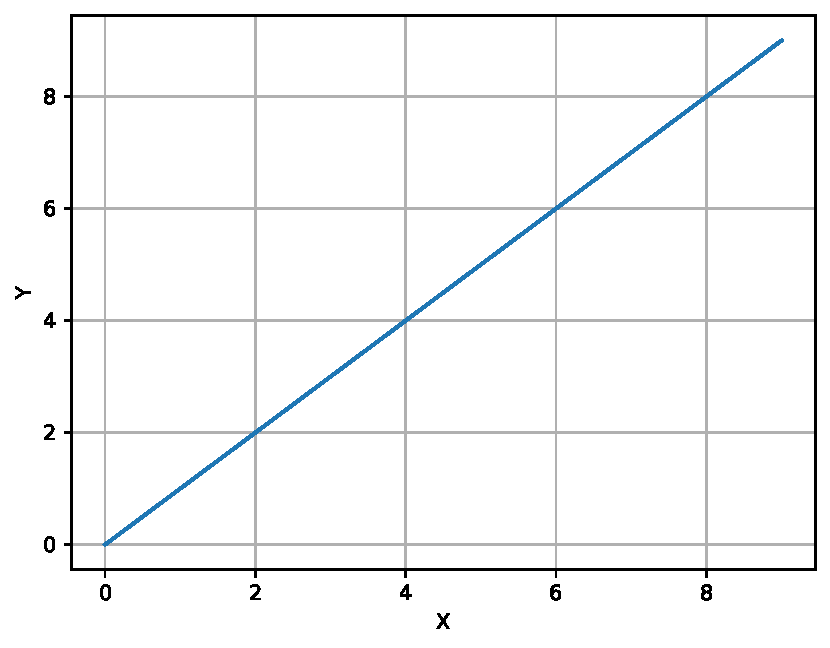
\includegraphics[scale=0.44]{figures/graph.pdf}
\caption{A graph}
\label{fig-agraph}
\end{figure}

Hier verwijs ik automatisch naar Figure \ref{fig-agraph}. \\
\todo{Hier maak ik een citaat, dat komt automatisch in de bibliography vanonder \cite{Becchetti06acomparison}.}
\section{Whales}
	Lorem ipsum dolor sit amet, consectetur adipiscing elit. Vestibulum laoreet dapibus purus. Maecenas eleifend, ipsum eget pretium blandit, nibh diam fermentum turpis, quis semper urna orci eget dolor. Aliquam at vehicula odio. Sed facilisis, odio vitae faucibus consequat, nisi metus condimentum leo, et malesuada sapien metus nec odio. Etiam vel orci non dolor interdum ultricies. Nullam in justo dui. Aenean ut eros non felis molestie lacinia eget ut turpis. Mauris malesuada efficitur libero, at volutpat arcu imperdiet ac. Vivamus gravida sodales felis, varius ultrices magna luctus sit amet. Donec blandit ante neque, at blandit dui vestibulum in. Nam vel lorem.


\end{multicols}
\bibliographystyle{plain}
\bibliography{references}
\end{document}